\documentclass[openany]{book}
\usepackage{lmodern}
\usepackage{amssymb,amsmath}
\usepackage{ifxetex,ifluatex}
\usepackage{fixltx2e} % provides \textsubscript
\ifnum 0\ifxetex 1\fi\ifluatex 1\fi=0 % if pdftex
  \usepackage[T1]{fontenc}
  \usepackage[utf8]{inputenc}
\else % if luatex or xelatex
  \ifxetex
    \usepackage{mathspec}
  \else
    \usepackage{fontspec}
  \fi
  \defaultfontfeatures{Ligatures=TeX,Scale=MatchLowercase}
\fi
% use upquote if available, for straight quotes in verbatim environments
\IfFileExists{upquote.sty}{\usepackage{upquote}}{}
% use microtype if available
\IfFileExists{microtype.sty}{%
\usepackage{microtype}
\UseMicrotypeSet[protrusion]{basicmath} % disable protrusion for tt fonts
}{}
\usepackage[margin=1in]{geometry}
\usepackage{hyperref}
\hypersetup{unicode=true,
            pdftitle={Singapore Society in Numbers},
            pdfauthor={Edited by Shannon Ang},
            pdfborder={0 0 0},
            breaklinks=true}
\urlstyle{same}  % don't use monospace font for urls
\usepackage{natbib}
\bibliographystyle{apalike}
\usepackage{color}
\usepackage{fancyvrb}
\newcommand{\VerbBar}{|}
\newcommand{\VERB}{\Verb[commandchars=\\\{\}]}
\DefineVerbatimEnvironment{Highlighting}{Verbatim}{commandchars=\\\{\}}
% Add ',fontsize=\small' for more characters per line
\usepackage{framed}
\definecolor{shadecolor}{RGB}{248,248,248}
\newenvironment{Shaded}{\begin{snugshade}}{\end{snugshade}}
\newcommand{\KeywordTok}[1]{\textcolor[rgb]{0.13,0.29,0.53}{\textbf{#1}}}
\newcommand{\DataTypeTok}[1]{\textcolor[rgb]{0.13,0.29,0.53}{#1}}
\newcommand{\DecValTok}[1]{\textcolor[rgb]{0.00,0.00,0.81}{#1}}
\newcommand{\BaseNTok}[1]{\textcolor[rgb]{0.00,0.00,0.81}{#1}}
\newcommand{\FloatTok}[1]{\textcolor[rgb]{0.00,0.00,0.81}{#1}}
\newcommand{\ConstantTok}[1]{\textcolor[rgb]{0.00,0.00,0.00}{#1}}
\newcommand{\CharTok}[1]{\textcolor[rgb]{0.31,0.60,0.02}{#1}}
\newcommand{\SpecialCharTok}[1]{\textcolor[rgb]{0.00,0.00,0.00}{#1}}
\newcommand{\StringTok}[1]{\textcolor[rgb]{0.31,0.60,0.02}{#1}}
\newcommand{\VerbatimStringTok}[1]{\textcolor[rgb]{0.31,0.60,0.02}{#1}}
\newcommand{\SpecialStringTok}[1]{\textcolor[rgb]{0.31,0.60,0.02}{#1}}
\newcommand{\ImportTok}[1]{#1}
\newcommand{\CommentTok}[1]{\textcolor[rgb]{0.56,0.35,0.01}{\textit{#1}}}
\newcommand{\DocumentationTok}[1]{\textcolor[rgb]{0.56,0.35,0.01}{\textbf{\textit{#1}}}}
\newcommand{\AnnotationTok}[1]{\textcolor[rgb]{0.56,0.35,0.01}{\textbf{\textit{#1}}}}
\newcommand{\CommentVarTok}[1]{\textcolor[rgb]{0.56,0.35,0.01}{\textbf{\textit{#1}}}}
\newcommand{\OtherTok}[1]{\textcolor[rgb]{0.56,0.35,0.01}{#1}}
\newcommand{\FunctionTok}[1]{\textcolor[rgb]{0.00,0.00,0.00}{#1}}
\newcommand{\VariableTok}[1]{\textcolor[rgb]{0.00,0.00,0.00}{#1}}
\newcommand{\ControlFlowTok}[1]{\textcolor[rgb]{0.13,0.29,0.53}{\textbf{#1}}}
\newcommand{\OperatorTok}[1]{\textcolor[rgb]{0.81,0.36,0.00}{\textbf{#1}}}
\newcommand{\BuiltInTok}[1]{#1}
\newcommand{\ExtensionTok}[1]{#1}
\newcommand{\PreprocessorTok}[1]{\textcolor[rgb]{0.56,0.35,0.01}{\textit{#1}}}
\newcommand{\AttributeTok}[1]{\textcolor[rgb]{0.77,0.63,0.00}{#1}}
\newcommand{\RegionMarkerTok}[1]{#1}
\newcommand{\InformationTok}[1]{\textcolor[rgb]{0.56,0.35,0.01}{\textbf{\textit{#1}}}}
\newcommand{\WarningTok}[1]{\textcolor[rgb]{0.56,0.35,0.01}{\textbf{\textit{#1}}}}
\newcommand{\AlertTok}[1]{\textcolor[rgb]{0.94,0.16,0.16}{#1}}
\newcommand{\ErrorTok}[1]{\textcolor[rgb]{0.64,0.00,0.00}{\textbf{#1}}}
\newcommand{\NormalTok}[1]{#1}
\usepackage{longtable,booktabs}
\usepackage{graphicx,grffile}
\makeatletter
\def\maxwidth{\ifdim\Gin@nat@width>\linewidth\linewidth\else\Gin@nat@width\fi}
\def\maxheight{\ifdim\Gin@nat@height>\textheight\textheight\else\Gin@nat@height\fi}
\makeatother
% Scale images if necessary, so that they will not overflow the page
% margins by default, and it is still possible to overwrite the defaults
% using explicit options in \includegraphics[width, height, ...]{}
\setkeys{Gin}{width=\maxwidth,height=\maxheight,keepaspectratio}
\IfFileExists{parskip.sty}{%
\usepackage{parskip}
}{% else
\setlength{\parindent}{0pt}
\setlength{\parskip}{6pt plus 2pt minus 1pt}
}
\setlength{\emergencystretch}{3em}  % prevent overfull lines
\providecommand{\tightlist}{%
  \setlength{\itemsep}{0pt}\setlength{\parskip}{0pt}}
\setcounter{secnumdepth}{5}
% Redefines (sub)paragraphs to behave more like sections
\ifx\paragraph\undefined\else
\let\oldparagraph\paragraph
\renewcommand{\paragraph}[1]{\oldparagraph{#1}\mbox{}}
\fi
\ifx\subparagraph\undefined\else
\let\oldsubparagraph\subparagraph
\renewcommand{\subparagraph}[1]{\oldsubparagraph{#1}\mbox{}}
\fi

%%% Use protect on footnotes to avoid problems with footnotes in titles
\let\rmarkdownfootnote\footnote%
\def\footnote{\protect\rmarkdownfootnote}

%%% Change title format to be more compact
\usepackage{titling}

% Create subtitle command for use in maketitle
\providecommand{\subtitle}[1]{
  \posttitle{
    \begin{center}\large#1\end{center}
    }
}

\setlength{\droptitle}{-2em}

  \title{Singapore Society in Numbers}
    \pretitle{\vspace{\droptitle}\centering\huge}
  \posttitle{\par}
    \author{Edited by Shannon Ang}
    \preauthor{\centering\large\emph}
  \postauthor{\par}
      \predate{\centering\large\emph}
  \postdate{\par}
    \date{Last updated 20 May 2019}

\usepackage{booktabs}
\usepackage{amsthm}
\makeatletter
\def\thm@space@setup{%
  \thm@preskip=8pt plus 2pt minus 4pt
  \thm@postskip=\thm@preskip
}
\makeatother

\begin{document}
\maketitle

{
\setcounter{tocdepth}{1}
\tableofcontents
}
\chapter*{Preface}\label{preface}
\addcontentsline{toc}{chapter}{Preface}

This online book is a compilation of resources aimed at advancing
quantitative social science in Singapore. It is meant to be a `living
document', so it will be updated as frequently as possible. The main
goal is to promote interest, rigour, and transparency in trying to
understand Singapore society quantitatively. It does so by:

\begin{enumerate}
\def\labelenumi{\arabic{enumi}.}
\tightlist
\item
  \textbf{Providing information on Singapore-relevant datasets} that are
  currently used to answer research and policy questions (Chapter
  \ref{publicdata} and Chapter \ref{restricteddata}). This includes:

  \begin{itemize}
  \tightlist
  \item
    Descriptions of \emph{publicly available} datasets and how to access
    them. This overview of the `data landscape' will be helpful for
    social scientists to get started with research on Singapore, and
    prevent wasteful overlap in primary data collection across
    institutions.
  \item
    A list of \emph{restricted} or \emph{non-publicly available}
    datasets that could be used to answer important research or policy
    questions if access was granted. If available, details on the
    dataset and reasons for data restriction will also be listed. It is
    hoped that this list will promote greater transparency in data
    sharing across research teams.
  \end{itemize}
\item
  \textbf{Maintaining a repository of replicable case studies on
  Singapore society} (with annotated code, where possible) which can be
  used for illustrations in any quantitatively oriented college-level
  class (Chapter \ref{races} to Chapter \ref{lifecourse}). These may be
  short summaries (blog-length) of published work, or side analyses that
  may not be appropriate for an academic journal but are useful for
  Singapore social science nonetheless.
\item
  \textbf{Occasional think pieces by researchers} on best practices and
  on how to improve quantitative social science in Singapore (Chapter
  \ref{think}).
\end{enumerate}

\section*{Why I started this project}\label{why-i-started-this-project}
\addcontentsline{toc}{section}{Why I started this project}

Quantitative research is not (and should not be) the only approach we
take to understanding Singapore society, but constant appeals to ``big
data''\footnote{See, for instance,
  \url{https://www.todayonline.com/singapore/business-big-data-singapore-has-built-cutting-edge}}
or claims of ``evidence-based policy''\footnote{Government agencies such
  as the Ministry of Social and Family Development often
  \href{https://www.msf.gov.sg/about-MSF/our-people/Divisions-at-MSF/Family-Development-and-Support/Pages/default.aspx}{use
  such a phrase}} makes it ever more important for members of the public
to \textbf{critically evaluate the use of numbers} in making arguments
or in representations of social phenomena.

Educational institutions have an important role to play in this
``data-driven'' world. Every year, undergraduates studying the social
sciences in our local universities take several courses in research
methods to fulfil the requirements of their degrees. Part of this
research methods sequence typically involves training in introductory
statistics or ``quantitative reasoning''. Quantitative courses in social
science departments differ from those taught in the natural sciences
because they are thought to be more applied - the focus is on the use of
statistical methods to answer questions about society. Understanding and
applying these methods \emph{to the Singapore context} is crucial here -
at this point, students learn (and hopefully are inspired) about the
kind of questions they can ask about the very society they live in,
given the quantitative tools they are learning.

However, my first exposure to statistics as an undergraduate reading
Sociology at NUS\footnote{(the) National University of Singapore} was to
textbooks containing examples only from Western societies
\citep[e.g.,][]{agresti_statistical_2009, treiman_quantitative_2009}.
While the use of these internationally-recognized textbooks may provide
some assurance of quality education, sole reliance on foreign material
often becomes a missed opportunity to inspire students to build on and
improve Singapore social science. Without contextualization\footnote{Notwithstanding
  the terribly unhelpful stereotype of social science students being
  ``good at writing but bad at numbers''.}, abstract statistical
concepts (e.g., hypotheses testing, chi-squared tests) seem removed from
everyday experience, and impede the ability to take these important
concepts beyond the classroom and into public dialogue.

I started this book with the view to use it primarily \emph{as a
teaching tool}\footnote{For instance, the public repository of
  Singapore-oriented examples and illustrations may be used to
  supplement courses based on textbooks written by international
  scholars.}, but it can be used in many other ways. It is hoped that in
the long term, resources in this book will encourage quantitative
literacy and research in Singapore by making it easier for interested
parties to browse and use with Singapore-relevant data. Social science
researchers may use the dataset listings as a springboard for
collaboration, or present their own interesting case studies for the
benefit of the Singapore public. Others (such as journalists, civil
servants, or non-profit organizations) may find value in these material
as a gateway to quantitative research on Singapore society, and how to
think about pertinent issues surrounding such work.

\section*{How to contribute}\label{how-to-contribute}
\addcontentsline{toc}{section}{How to contribute}

Instructions on how to list a dataset, contribute a case study, or write
a think piece for this page.

\section*{Acknowledgements}\label{acknowledgements}
\addcontentsline{toc}{section}{Acknowledgements}

This book is being written through the \textbf{bookdown} package
\citep{R-bookdown}, which was built on top of R Markdown and
\textbf{knitr} \citep{xie2015}.

\section*{About me}\label{about-me}
\addcontentsline{toc}{section}{About me}

Little write-up about myself

Contributors

\part{Datasets for Social
Science}\label{part-datasets-for-social-science}

\chapter{Public Data}\label{publicdata}

List of public data

\chapter{Restricted Data}\label{restricteddata}

List of restricted data

\part{Case Studies}\label{part-case-studies}

\chapter{Race}\label{races}

This is a section on race

\section{Witty title for Case 1}\label{witty-title-for-case-1}

This is an example of in-line code annotation and output.

\begin{Shaded}
\begin{Highlighting}[]
\KeywordTok{par}\NormalTok{(}\DataTypeTok{mar =} \KeywordTok{c}\NormalTok{(}\DecValTok{4}\NormalTok{, }\DecValTok{4}\NormalTok{, .}\DecValTok{1}\NormalTok{, .}\DecValTok{1}\NormalTok{))}
\KeywordTok{plot}\NormalTok{(pressure, }\DataTypeTok{type =} \StringTok{'b'}\NormalTok{, }\DataTypeTok{pch =} \DecValTok{19}\NormalTok{)}
\end{Highlighting}
\end{Shaded}

\begin{figure}

{\centering 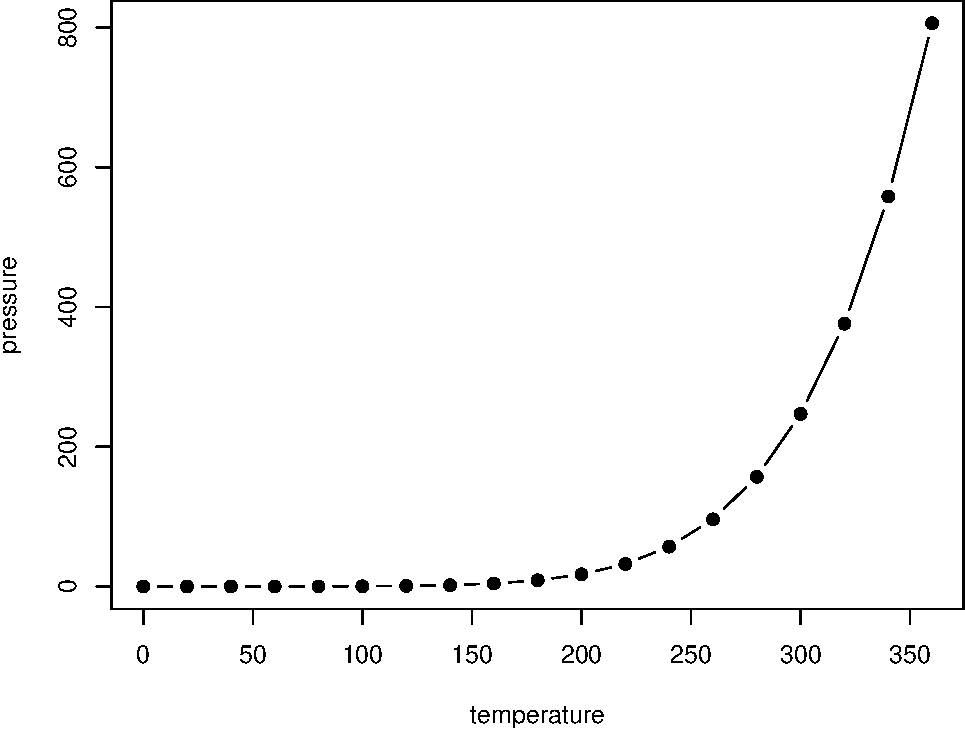
\includegraphics[width=0.8\linewidth]{bookdown_files/figure-latex/nice-fig-1} 

}

\caption{Here is a nice figure!}\label{fig:nice-fig}
\end{figure}

Figures can be referenced, e.g., see Figure \ref{fig:nice-fig}.
Similarly, you can reference tables generated from
\texttt{knitr::kable()}, e.g., see Table \ref{tab:nice-tab}.

\begin{Shaded}
\begin{Highlighting}[]
\NormalTok{knitr}\OperatorTok{::}\KeywordTok{kable}\NormalTok{(}
  \KeywordTok{head}\NormalTok{(iris, }\DecValTok{20}\NormalTok{), }\DataTypeTok{caption =} \StringTok{'Here is a nice table!'}\NormalTok{,}
  \DataTypeTok{booktabs =} \OtherTok{TRUE}
\NormalTok{)}
\end{Highlighting}
\end{Shaded}

\begin{table}[t]

\caption{\label{tab:nice-tab}Here is a nice table!}
\centering
\begin{tabular}{rrrrl}
\toprule
Sepal.Length & Sepal.Width & Petal.Length & Petal.Width & Species\\
\midrule
5.1 & 3.5 & 1.4 & 0.2 & setosa\\
4.9 & 3.0 & 1.4 & 0.2 & setosa\\
4.7 & 3.2 & 1.3 & 0.2 & setosa\\
4.6 & 3.1 & 1.5 & 0.2 & setosa\\
5.0 & 3.6 & 1.4 & 0.2 & setosa\\
\addlinespace
5.4 & 3.9 & 1.7 & 0.4 & setosa\\
4.6 & 3.4 & 1.4 & 0.3 & setosa\\
5.0 & 3.4 & 1.5 & 0.2 & setosa\\
4.4 & 2.9 & 1.4 & 0.2 & setosa\\
4.9 & 3.1 & 1.5 & 0.1 & setosa\\
\addlinespace
5.4 & 3.7 & 1.5 & 0.2 & setosa\\
4.8 & 3.4 & 1.6 & 0.2 & setosa\\
4.8 & 3.0 & 1.4 & 0.1 & setosa\\
4.3 & 3.0 & 1.1 & 0.1 & setosa\\
5.8 & 4.0 & 1.2 & 0.2 & setosa\\
\addlinespace
5.7 & 4.4 & 1.5 & 0.4 & setosa\\
5.4 & 3.9 & 1.3 & 0.4 & setosa\\
5.1 & 3.5 & 1.4 & 0.3 & setosa\\
5.7 & 3.8 & 1.7 & 0.3 & setosa\\
5.1 & 3.8 & 1.5 & 0.3 & setosa\\
\bottomrule
\end{tabular}
\end{table}

\chapter{Gender}\label{gender}

Gender sections

\section{Example one}\label{example-one}

\section{Example two}\label{example-two}

\chapter{Class / SES}\label{class}

Class section.

\section{Example one}\label{example-one-1}

\section{Example two}\label{example-two-1}

\chapter{Religion}\label{religion}

Religion section

\section{Example 1}\label{example-1}

\chapter{Life Course}\label{lifecourse}

Life course sections

\part{Think Pieces}\label{part-think-pieces}

\chapter{Thinking about Numbers}\label{think}

Think pieces section

\section{Think piece 1}\label{think-piece-1}

\bibliography{book.bib,packages.bib,zotero.bib}


\end{document}
